\section{Problem Formulation}
\paragraph{LLM Reasoning.} A finite-horizon MDP $\mathcal{M}$ can be defined by the state space $\mathcal{S}$, action space $\mathcal{A}$, horizon $T$, and reward function $r_{\mathcal{M}}(s, a)$, where $s\in\mathcal{S}$ and $a\in\mathcal{A}$. Here, the initial state $s_0$ is the prompt, and the action $a_t$ is the $t$-th step of the CoT, which can be either separated by special tokens \citep{wang2023math} or defined as a fixed length of reasoning tokens \citep{luo2024improve}. We adopt the latter definition due to its simplicity. The state transition is deterministic by appending the new reasoning step, i.e., $s_{t+1} = s_t + a_t$.

We are interested in a training-deployment procedure. During training, the agent only receives information about the true MDP $\mathcal{M}^*\coloneqq (\mathcal{S}, \mathcal{A}, r, T)$ via the input training data $\mathcal{D}$. During deployment, we freeze the learned policy and deploy it in $\mathcal{M}^*$. Notably, $\mathcal{D}$ does not uniquely identify $\mathcal{M}^*$, inducing epistemic uncertainty about the MDP. Formally, $\mathcal{D}$ and a prior distribution over MDPs $p(\mathcal{M})$ define a posterior distribution over MDPs, $p(\mathcal{M}|\mathcal{D})\propto p(\mathcal{M})p(\mathcal{\mathcal{D}|\mathcal{M}})$. The objective for policy $\pi$ is thus to maximize return in expectation over MDPs from the posterior $p(\mathcal{M}|\mathcal{D})$:
\#\label{eq_org_obj}
\mathcal{J}(\pi) = \EE_{\mathcal{M}\sim p(\mathcal{M}\mid\mathcal{D})}\Bigl[\mathcal{J}_{\mathcal{M}}(\pi)\Bigr], \,\,\,\, \text{where } \mathcal{J}_{\mathcal{M}}(\pi) = \EE_{s_0, \pi}\Biggl[\sum_{t=0}^{T-1} r_{\mathcal{M}}(s_t, a_t)\Biggr].
\#
This $\mathcal{J}(\pi)$ objective is designed to, for any data $\mathcal{D}$, train a policy $\pi$ that maximizes its Bayes-expected return in the unknown true environment during deployment, i.e., its performance averaged over MDPs drawn from the posterior $p(\mathcal{M}|\mathcal{D})$.
\vspace{-0.15cm}
\paragraph{Progress Reward.} Prior work \citep{uesato2022solving,guo2025deepseek} employs an outcome-level reward $\text{verifier}(s_{T}, y_{s_0}^*)$ for the true MDP $\mathcal{M}^*$, which uses a verifier to perform a regular expression match (either $0$ or $1$) between $s_{T}$ and the ground-truth answer $y_{s_0}^*$ corresponding to the prompt $s_0$. 
We extend this sparse-reward setting by incorporating a \textit{progress} reward \citep{setlur2024rewarding,qu2025optimizing}, which quantifies the increase of the model's probability of outputting $y_{s_0}^*$ after appending $a$ at the CoT $s$, i.e., for $0\leq t\leq T-1$:
\#\label{def_r}
r(s_t, a_t) = \pi_{\phi}(y_{s_0}^*\mid s_t + a_t + \text{</think>}) - \pi_{\phi}(y_{s_0}^*\mid s_t + \text{</think>}),
\#
where </think> is the end sign of thinking, such as the answer elicitation prompt ``Based on the above reasoning, the answer is \texttt{\textbackslash boxed}'' that we adopt, and $\pi_\phi$ is any policy. Compared to Monte-Carlo process rewards \citep{luo2024improve,qu2025optimizing}, \eqref{def_r} is computationally efficient by avoiding multiple branched rollouts at each step, and the KV cache of $s_{0:T}$ during rollouts can also be reused. The above definition naturally extends to any $r_\mathcal{M}$ defined w.r.t. the answer $y_{s_0}^{\mathcal{M}}$. The Q-value is then
\#\label{def_q_m}
Q^{\pi}_\mathcal{M}(h_t, a_t) &= \EE_{\pi}\Biggl[\sum_{t'=t}^{T-1}r_{\mathcal{M}}(s_{t'}, a_{t'}) + \text{verifier}(s_T, y_{s_0}^*)\Biggr],
\#
where $h_t = (s_0, a_0, r_0, \ldots, s_t)$ is the history and we define $s(h_t) =s_t$ as the final state $s_t$ from $h_t$.

\begin{wrapfigure}{r}{0.2\textwidth}
        \vspace{-0.4cm}
    \begin{minipage}[t]{0.2\textwidth}
        \centering
        \begin{minipage}[t]{\linewidth}
            \centering
            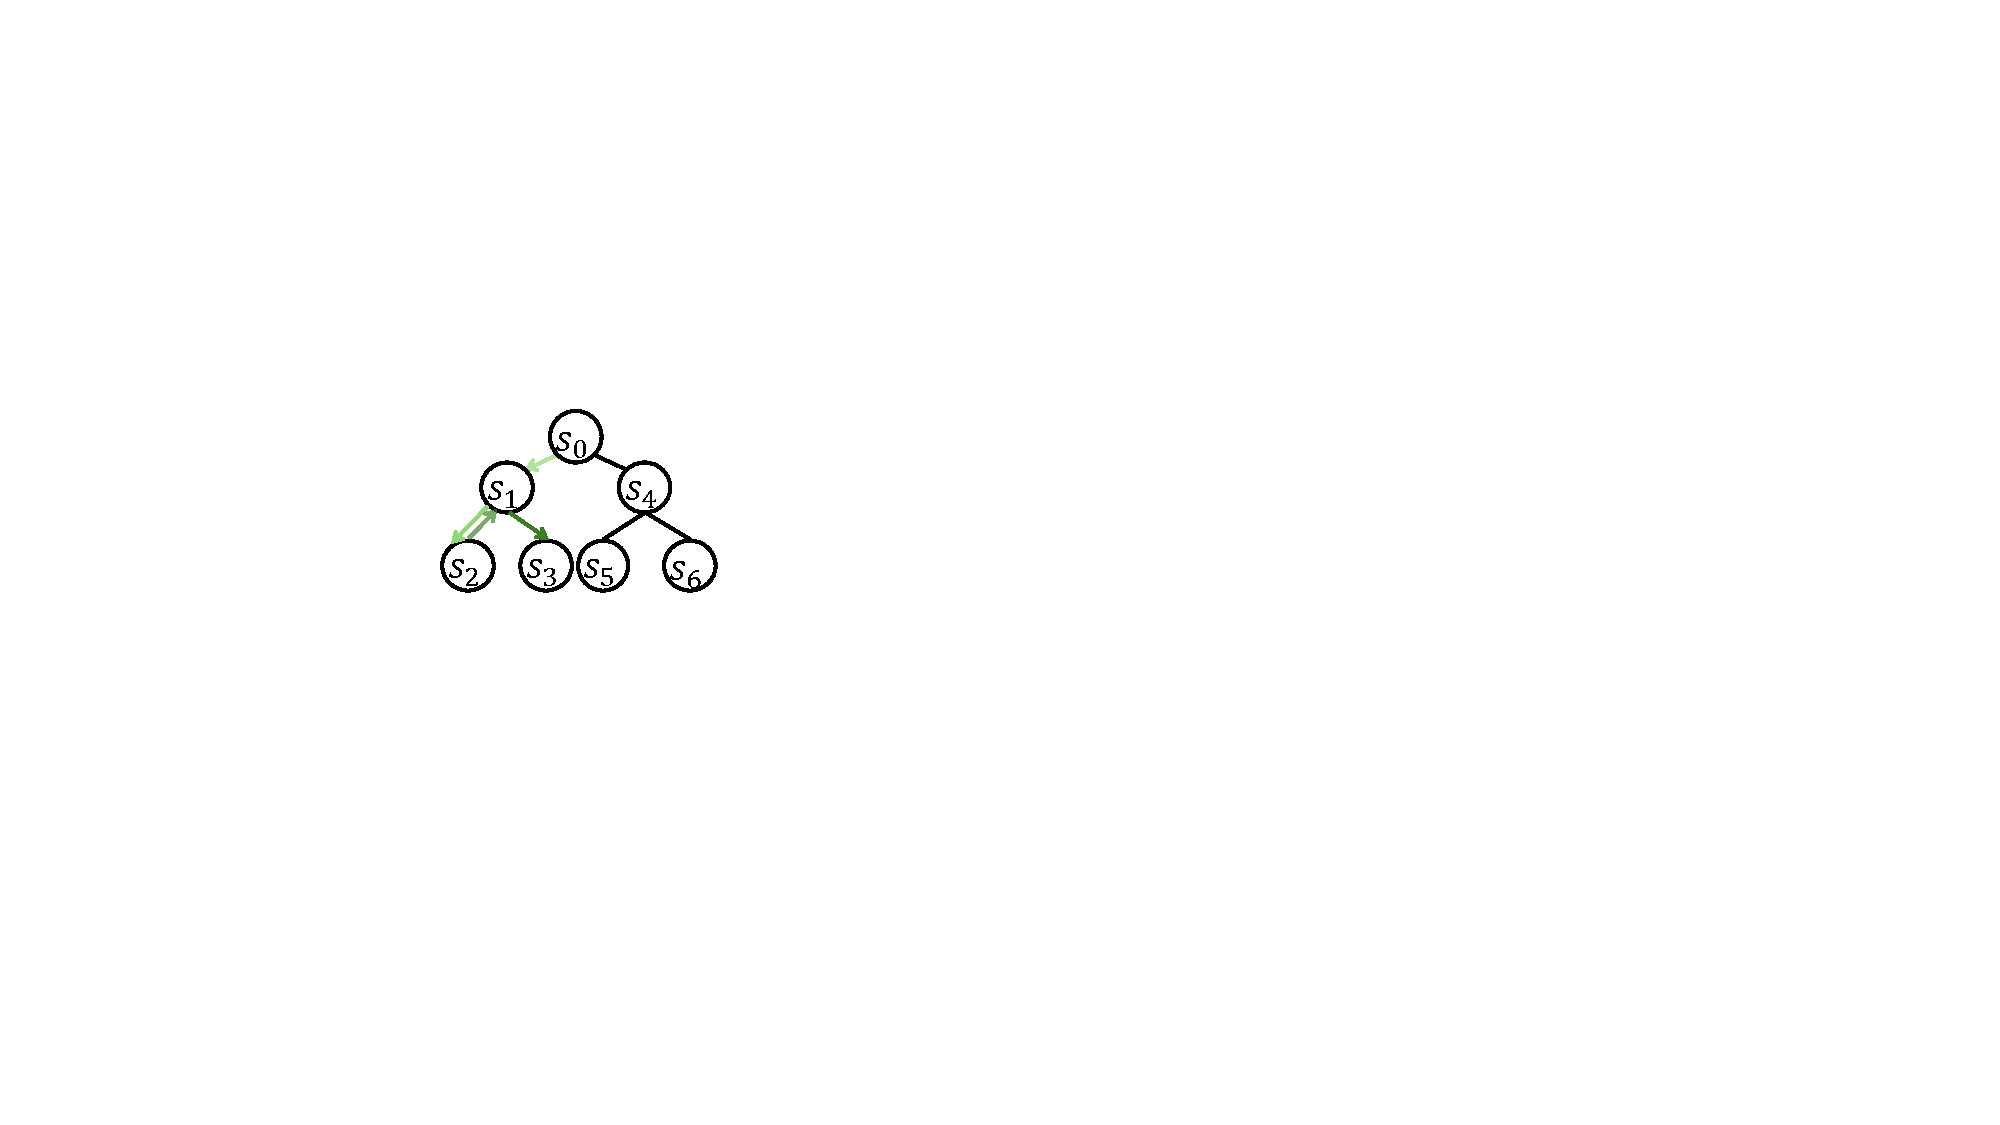
\includegraphics[width=\linewidth]{figs/binary_tree.pdf}
        \end{minipage}
        \vspace{-0.5cm}
        \setlength{\belowcaptionskip}{-10pt}
        \caption{An example of reflective reasoning trajectories.}
        \label{fig_binary_tree}
    \end{minipage}
\end{wrapfigure}
\vspace{-0.15cm}
\paragraph{Reflective Exploration.} Informally, we define reflective exploration as the pattern in which the LLM revisits a prior state after an exploratory step to take different actions at that state. Specifically, a language reflection step such as ``Let's reconsider the geometric relationship'' corresponds to revisiting and retrying. We illustrate this using a binary search tree as in the right figure: for the trajectory $s_0\shortrightarrow s_1\shortrightarrow s_2\shortrightarrow s_1\shortrightarrow s_3$, $s_1\shortrightarrow s_2$ is an exploration step, $s_2\shortrightarrow s_1$ is a reflective step that signals the strategy switch from $s_2$ to $s_3$, and the ``geometric relationship'' in the above example originates from $s_1$. We formalize this behavior through the lens of adaptive policies.

\begin{definition}[Uncertainty-Adaptive Policy]\label{def_uapi}
Define the belief as the posterior over MDPs $b(h_t)(\mathcal{M}) \coloneqq p(\mathcal{M} \mid h_t, \mathcal{D})$.
A policy $\pi$ is \emph{uncertainty-adaptive} if there exists a measurable mapping $\mu: \mathcal{S} \times \mathcal{P}(\mathcal{M}) \to \Delta(\mathcal{A})$ such that for all $h_t$ and $a_t$, $\pi(a_t\mid h_t)=\mu(a_t \mid s(h_t), b(h_t))$. If in addition, there exists $h_t$ and $h_t'$ such that $s(h_t)=s(h_t')$ but $\mu(a_t \mid s(h_t), b(h_t))\neq\mu(a_t \mid s(h_t'), b(h_t'))$, then $\pi$ is \emph{strictly} uncertainty-adaptive, or equivalently, not Markovian.
\end{definition}
From this perspective, reflective exploration is the behavioral signature of an uncertainty-adaptive policy: as the agent’s belief evolves, it rationally revisits previous states and generates a different action distribution. In contrast, a purely state-only policy that ignores this evolving belief would respond identically upon revisiting the same state. Formally,

\begin{definition}[Reflective Exploration]\label{def:reflective}
We say that a policy $\pi$ exhibits \emph{reflective exploration} if there exist $t_1> t_2$ and $h_{t_1}$, $h_{t_2}$ such that
\$
\varphi(s(h_{t_1})) = \varphi(s(h_{t_2})), \qquad \pi(\cdot \mid h_{t_1}) \neq \pi(\cdot \mid h_{t_2}),
\$
where $\varphi: \mathcal{S} \to \mathcal{Z}$ is a measurable mapping for which there exists $\vartheta: \mathcal{Z} \times \mathcal{H}_{\mathcal{R}} \to \Delta(\mathcal{A})$ satisfying for every $h_t$ that (1) $\vartheta(\cdot \mid \varphi(s_{t}), r_{0:t-1})= \pi(\cdot\mid h_t)$; and (2) if there is some process $X_t$ and some $\upsilon$ such that $\pi(\cdot\mid h_t) = \upsilon(\cdot\mid X_t)$ then $X_t = \psi(\varphi(s_t))$ for some measurable $\psi$.
\end{definition}
Intuitively, it describes an agent that returns to the same underlying latent state but, in light of what it has learned from past rewards, deliberately chooses a different strategy than it did before. The latent state representation $\varphi$ abstracts away superficial differences in the text state. The existence of $\vartheta$ and $\upsilon$, $\psi$ formalizes the latent factorization and state-minimality properties of $\varphi$, respectively. 